\documentclass[tikz]{standalone}
\usepackage{bm}
\usetikzlibrary{calc, bending, arrows.meta, shapes, backgrounds}
\definecolor{verde}{RGB}{181,200,182}
\definecolor{azzurro}{RGB}{189,217,255}

\begin{document}
	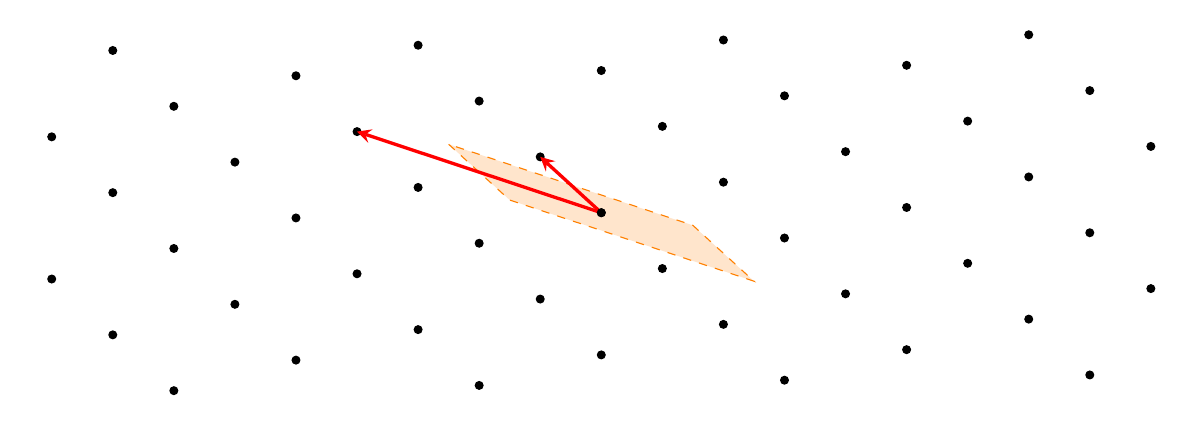
\begin{tikzpicture}[scale=0.47]
		\clip (-15.5,-5) rectangle (15.5, 5);
		\coordinate (Origin)   at (0,0);
		\coordinate (XAxisMin) at (-20,0);
		\coordinate (XAxisMax) at (20,0);
		\coordinate (YAxisMin) at (0,-20);
		\coordinate (YAxisMax) at (0,20);
		
		\def\scale{1.65}
		\def\bxOne{-4}   % b1 x-component
		\def\byOne{1.32842712} % b1 y-component
		\def\bxTwo{-1} % b2 x-component
		\def\byTwo{0.91421356}   % b2 y-component
		
		
		\coordinate (hb1) at ({0.5*\scale*\bxOne}, {0.5*\scale*\byOne});
		\coordinate (hb2) at ({0.5*\scale*\bxTwo}, {0.5*\scale*\byTwo});
		
		%\foreach \i in {-6,...,6}{
		%	\foreach \j in {-15,...,15}{
				% Center point: lattice site
		%		\pgfmathsetmacro{\x}{\scale*(\i*\bxOne + \j*\bxTwo)}
		%		\pgfmathsetmacro{\y}{\scale*(\i*\byOne + \j*\byTwo)}
		%		\coordinate (P) at (\x,\y);
				
				% Corners: P ± ½b₁ ± ½b₂
		%		\coordinate (A) at ($ (P) + (hb1) + (hb2) $);
		%		\coordinate (B) at ($ (P) + (hb1) - (hb2) $);
		%		\coordinate (C) at ($ (P) - (hb1) - (hb2) $);
		%		\coordinate (D) at ($ (P) - (hb1) + (hb2) $);
				
				% Draw filled parallelogram
		%		\draw[draw=red!20] (A) -- (B) -- (C) -- (D) -- cycle;
		%	}
		%}
		
		% Highlight the centered fundamental parallelogram at (0,0)
		\coordinate (O) at (0,0);
		\coordinate (hb1) at ({0.5*\scale*\bxOne}, {0.5*\scale*\byOne});
		\coordinate (hb2) at ({0.5*\scale*\bxTwo}, {0.5*\scale*\byTwo});
		
		\coordinate (HA) at ($ (O) + (hb1) + (hb2) $);
		\coordinate (HB) at ($ (O) + (hb1) - (hb2) $);
		\coordinate (HC) at ($ (O) - (hb1) - (hb2) $);
		\coordinate (HD) at ($ (O) - (hb1) + (hb2) $);
		
		\draw[dashed, orange, fill=orange!20] (HA) -- (HB) -- (HC) -- (HD) -- cycle;
		
		%\draw [very thin, gray!50,] (XAxisMin) -- (XAxisMax);% Draw x axis
		%\draw [very thin, gray!50,] (YAxisMin) -- (YAxisMax);% Draw y axis
		
		
		
		\foreach \i in {-11,...,11}{
			\foreach \j in {-15,...,15}{
				\pgfmathsetmacro{\x}{\scale*(\i*\bxOne + \j*\bxTwo)}
				\pgfmathsetmacro{\y}{\scale*(\i*\byOne + \j*\byTwo)}
				\node[draw,circle,inner sep=1pt,fill] at (\x, \y) {};
			}
		}
		
		\draw [draw=red!100, -stealth, very thick] (0,0) -- (\scale*\bxOne,\scale*\byOne) node [above] {};
		\draw [draw=red!100, -stealth, very thick] (0,0) -- (\scale*\bxTwo,\scale*\byTwo) node [left] {};
		
		\node[draw,circle,inner sep=1pt,fill] at (0,0) {};
		
	\end{tikzpicture}
\end{document}